\subsection{Diseño de la Fuente de Alimentación Lineal}
\bigskip 

En líneas generales, todo el amplificador estará alimentado por cuatro rieles, dos de alta tensión y dos de baja. Los rieles de altas serán suministrados por una fuente lineal mientras que para los de bajas, se reducirá la tensión de los rieles altos con una fuente conmutada. En esta sección se detallara el diseño de la fuente lineal. La misma consiste esencialmente de tres bloques:

\begin{itemize}
\item Transformador 220/36+36
\item Rectificador de onda completa
\item Divisor capacitivo 
\end{itemize}

El transformador reduce de 220$V_{rms}$ a 72$V_{rms}$, es decir, tensión pico de $72V_{rms}*\sqrt{2}=101.82V$.

Para el rectificador de onda completa se usaron diodos 6A10 en paralelo con capacitores de $100nF$ para reducir ruido. La caída en los diodos es de aproximadamente $0.7V$, reduciendo la tensión a la salida de este bloque a $101.82V-2*0.7V=100.4V$

Finalmente para el divisor capacitivo, se colocaron dos hileras de capacitores en paralelo, dando un divisor de $2200{\mu}F*4=8800{\mu}F$. El punto medio del divisor toma la tension de tierra, y los otros, $\pm50.2V$.


\begin{figure}[H]
\centering
\centerline{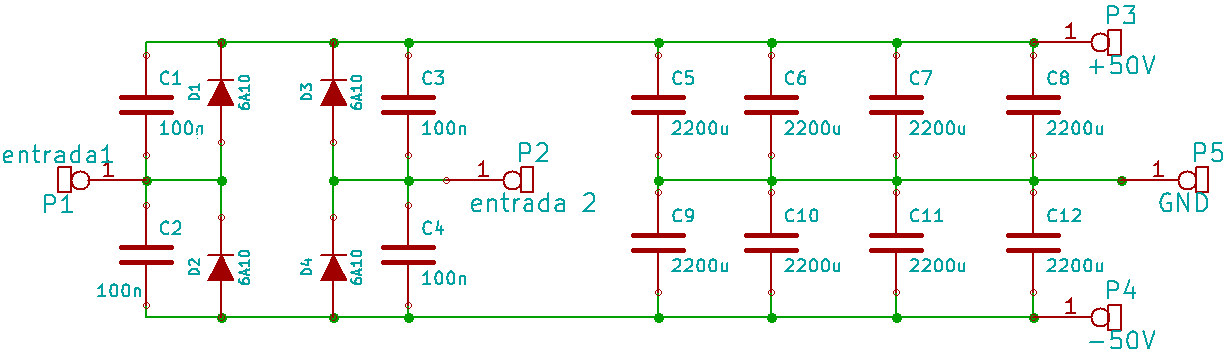
\includegraphics[scale=0.4]{img/esquema_fuente_lineal.png}}
\caption{Esquema de la fuente lineal}
\label{esquema_fuente_lineal} 
\end{figure}

\subsubsection*{Ripple}

Para calcular el factor de rizado $F_r=\frac{V_{ca}}{V_{cd}}$ vamos a separar los casos entre el riel alto y el bajo, porque no ven la misma carga.

El riel alto ademas de ver el amplificador, alimenta la fuente de switching, así que las impedancias de entrada quedan en paralelo, empeorando el factor de ripple. Aproximadamente la impedancia de entrada de la switching son $500\ohm$, despreciando todo menos la resistencia en serie que se ve del bobinado del relé y el bobinado del primario. Luego, $500\ohm$ en paralelo con la resistencia de entrada simulada del amplificador $1.8k\ohm$ es aproximadamente $400\ohm$.Ve también un capacitor de $220{\mu}F$.
Por tanto, el factor de rizado queda:

\[
	F_r=\frac{1}{\sqrt{3}(4fRC-1)}$$
$$	F_r=\frac{1}{\sqrt{3}(4\times 50Hz\times 400\ohm\times (8800+220){\mu}F-1)}$$
$$	F_r=0.00046
\]

El riel bajo ve aproximadamente $R_i=\frac{-50V}{-25mA}=2k\ohm$, valor de corriente obtenido por simulación sin señal. Ve también un capacitor de $220{\mu}F$.
Por tanto, el factor de rizado queda:

\[
	F_r=\frac{1}{\sqrt{3}(4fRC-1)}$$
$$	F_r=\frac{1}{\sqrt{3}(4\times 50Hz\times 2k\ohm\times (8800+220){\mu}F-1)}$$
$$	F_r=0.00016
\]

Para el peor caso de carga, es decir con una entrada de $V_i=1V_{rms}$, la carga vista será $R_i=\frac{-50V}{-4A}=12.5\ohm$ y $F_r=0.026$ en el pico del semiciclo negativo. Este caso será sumamente inusual de ver.

\subsection{Fuente Conmutada}

Para este tipo de fuente utilizaremos la topología Flyback con dos salidas, debido a su sencillez y bajo costo, su esquema puede observarse en la Figura~\ref{topo_flyback}. se Utilizaron dos bobinas de salida para generar 20V c/u; aprovechando el aislamiento galvánico generado por las bobinas acopladas se conectaron de forma tal de obtener dos bornes de $\pm 20V$, como se observa en la Figura~\ref{conmutada_basica} . Para controlar el ancho del pulso que activa el mosfet se utilizo un TL494, con un divisor a la salida para reescalar a una tension que el integrado pueda manejar fácilmente.

\begin{figure}[H]
\centering
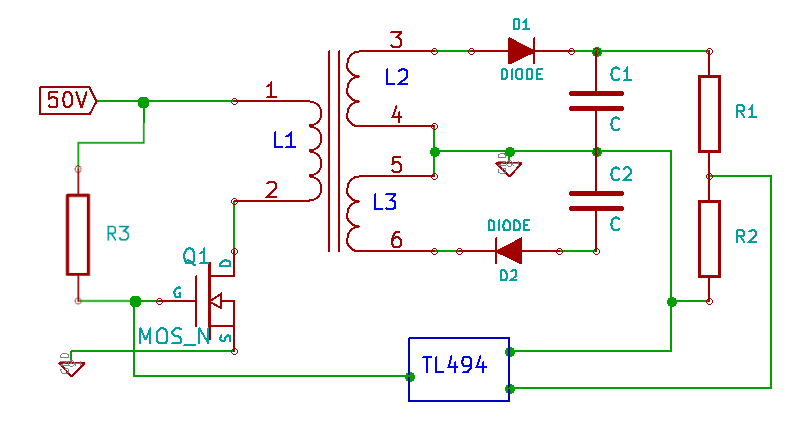
\includegraphics[width=0.90\textwidth]{img/conmutada_basica.png}
\caption{Esquema  basico fuente conmutada.}
\label{conmutada_basica}
\end{figure}

\subsubsection{Controlador}

Se utilizó el circuito integrado TL494 como circuito de control de la fuente conmutada. El metodo de control es mediante la modulación del ancho de pulso. 
